Here, we discuss the process of converting the face embedding (\emph{latent vector}) to a complete face image using \texttt{StyleGAN2} (our chosen generative model). We discuss our reasons for choosing this particular architecture and how we use it.

\begin{figure}[H]
    \centering
    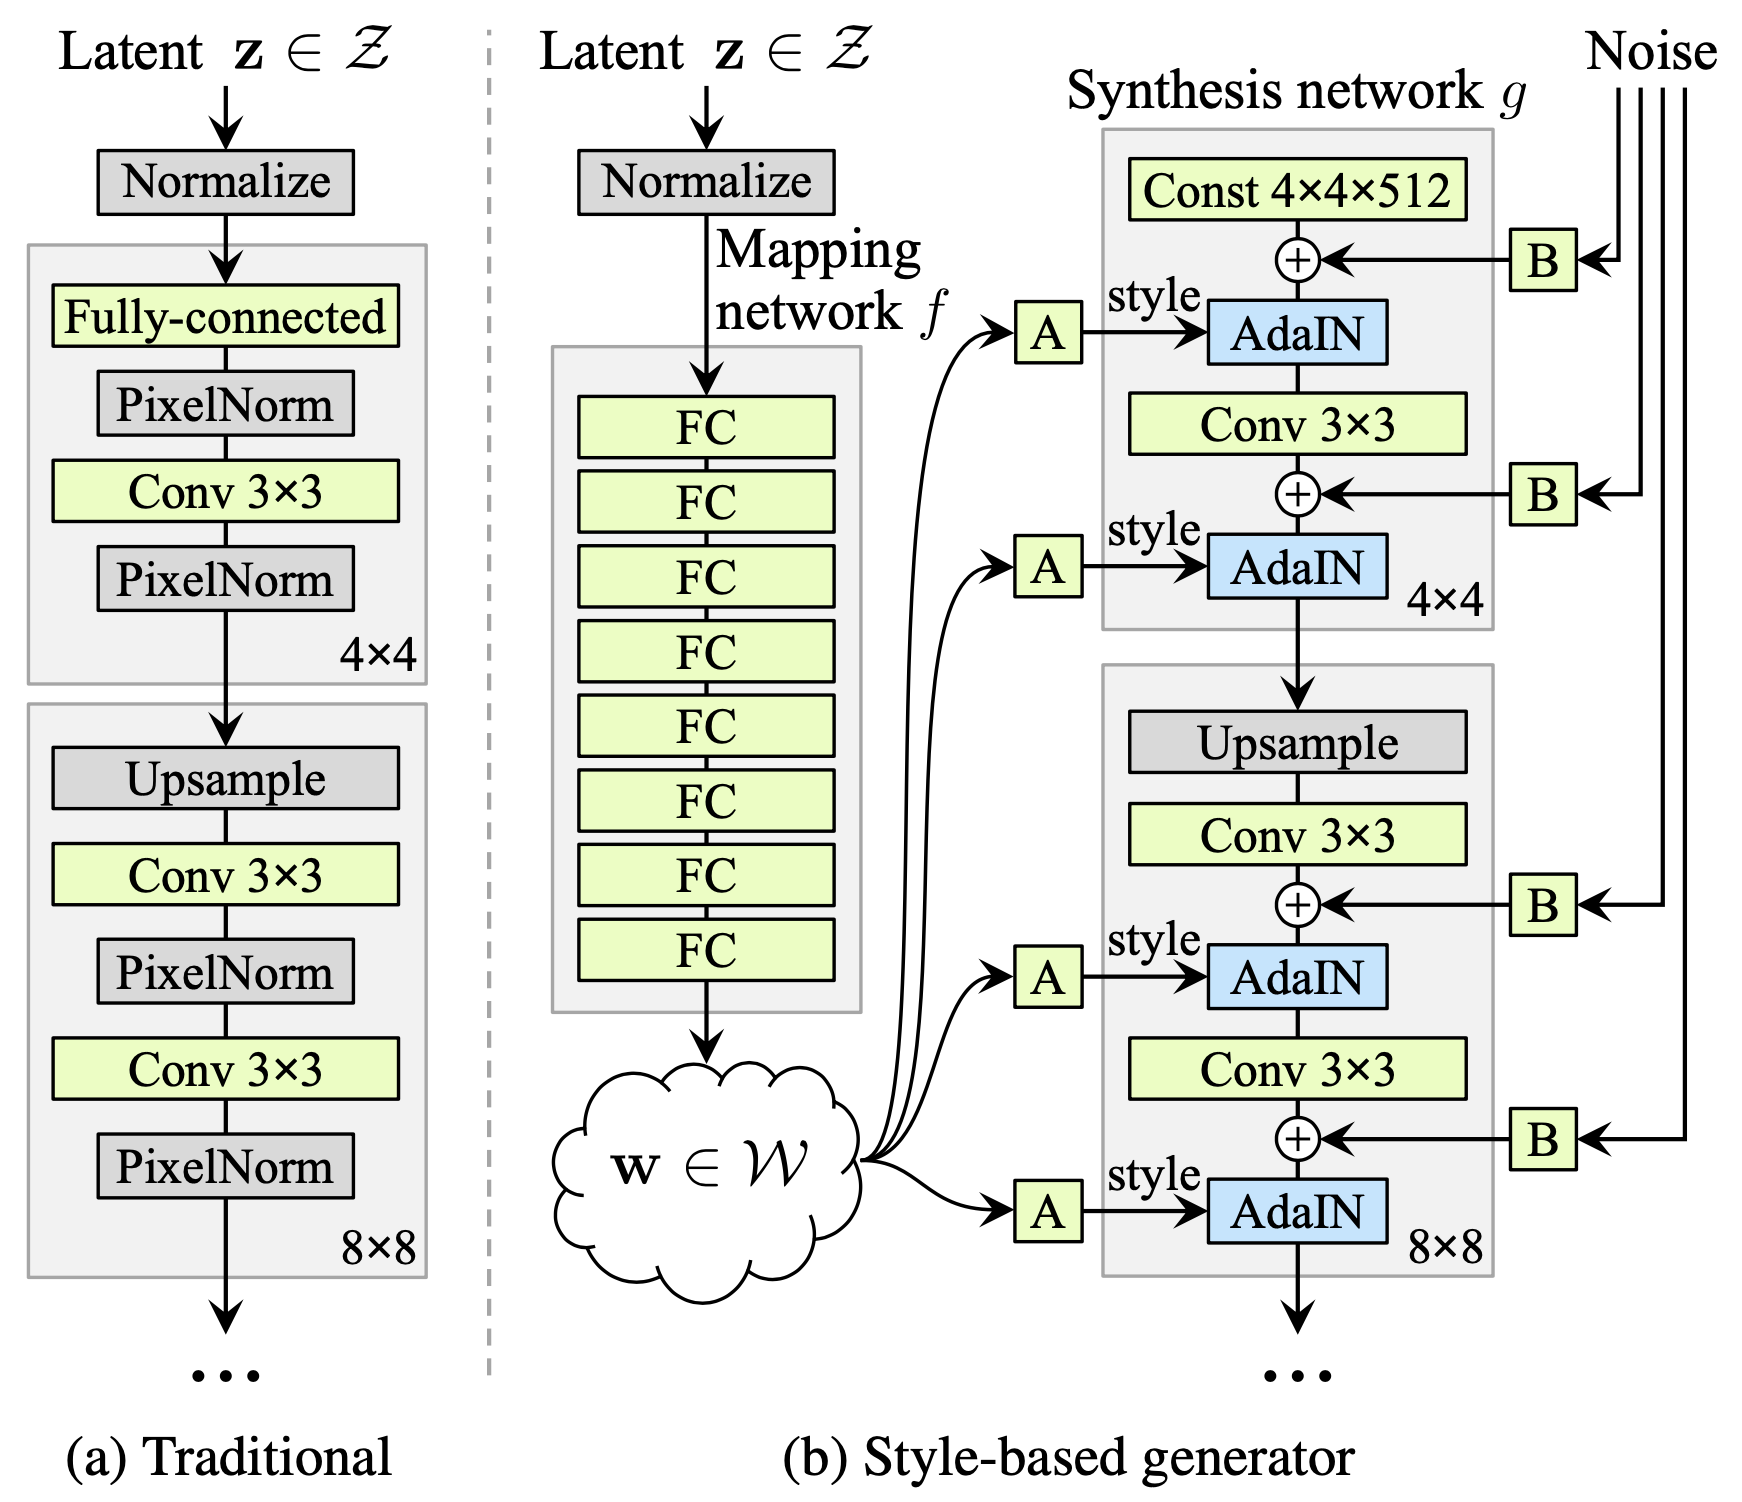
\includegraphics[width=0.7\textwidth]{images/stylegan.png}
    \caption{Style-based GAN architecture against traditional GAN}
    \label{fig:stylegan}
\end{figure}

\subsubsection{Functional Description}

This module utilizes the power of \emph{style-based} generative models, specifically \texttt{StyleGAN2} \cite{karras2020analyzing}, to translate the required \emph{latent vector} to a complete \emph{human face image}. \emph{Style-based GANs} (sometimes called \emph{latent-based GANs}) can exert artistic control over the generated content (images, videos, text ..., etc). Consequently, we can tune it to fit our need and, iteratively, design it along with \emph{code generation} \ref{sec:code_gen} and \emph{text processing} \ref{sec:text}, in order to have a complete end-to-end pipeline for \emph{text-to-face generation}.

\begin{itemize}
    \item \textbf{Input :}
    \begin{itemize}
        \item Low dimensional face embedding vector (latent vector).
    \end{itemize}
    \item \textbf{Output :}
    \begin{itemize}
        \item Complete human face image (portrait).
    \end{itemize}
\end{itemize}

\subsubsection{Modular Decomposition}

As mentioned before, we opt to use \emph{Style-based GANs} to be able to artistically control the output and designed the whole pipeline for \emph{text-to-face generation}. Moreover, we choose \texttt{StyleGAN2}, because it's one of the most popular and robust Style-based GANs in research literature. Also, it's relatively lightweight compared to other GANs used for the same purposes, but most importantly, \texttt{StyleGAN2} excels at human face generation based on latent space. Figure \ref{fig:stylegan} shows the original architecture of \texttt{StyleGAN} and how it is compared to traditional GANs. \texttt{StyleGAN} generator has two networks as follows :

\begin{itemize}
    \item \textbf{Mapping network} creates nonlinear transformation to the input latent vector $z$ ($512D$). This transformation is not invertible and results in a $512D$ latent vector $w$. This latent vector $w$ is expanded into several $512D$ vector using affine transformation, which gives the \emph{extended latent vector} $w+$. The extended latent vector $w+$ dimensions depend on the dimensions of the output image.
    \item \textbf{Synthesis network} generates the synthetic image from \emph{normally-distributed noise} guided by the extended latent vector $w+$.
\end{itemize}

\texttt{StyleGAN2} \cite{karras2020analyzing} is a newer version that follows the same architecture, but with some modifications to further improve the control over latent space and the quality of the outputs. 

So, let's discuss how we adapted \texttt{StyleGAN2} to our work :

\begin{itemize}
    \item To provide a high fidelity results, we target $1024X1024$ synthetic images. To achieve this, we have to use an extended latent vector $w+$ of dimensions $18X512$, meaning we repeat the latent vector $w$ $18$ times with \emph{affine transformation} for each.
    \item To further improve feature directions disentanglement, we fine-tune \texttt{StyleGAN2} using a subset of \texttt{FFHQ} dataset with increasing the weight of \emph{perceptual path regularization} in the loss function. \emph{Perceptual path regularization} in \texttt{StyleGAN2} loss encourages the smooth mapping between latent and image spaces. So, when increasing it in certain directions, it highly penalizes the deviation between latent and image spaces in these directions giving more organized latent space. To avoid using the whole dataset, we use \texttt{StyleGAN2} \emph{adaptive discriminator augmentation} (\textbf{ADA}) \cite{karras2020training} training methodology.
    \item Finally, we opt to remove the \emph{mapping network} of \emph{StyleGAN2} generator and only use the \emph{synthesis network}. This is mainly because :
    \begin{itemize}
        \item The mapping network doesn't satisfy the \emph{path length regularization}, so there is no smooth mapping between latent space $z$ and image space (only with latent space $w$). This is discussed in the original paper \cite{karras2020analyzing} and our experiments support that.
        \item The mapping network is not invertible, unlike the synthesis network. So, we cannot reverse the transformation from image space to latent space $z$. That's why we only work with latent space $w$ to test the consistency of the results.
        \item Removing the mapping network reduces the computations and the memory footprint, which is crucial in our case.
    \end{itemize}
\end{itemize}

After the previous modifications, the output model can directly translate the face embedding vector (\emph{latent space}) into a complete human face portrait.

\subsubsection{Design Constraints}

The basic design constraints for this module can be enumerated as follows :

\begin{enumerate}
    \item \textbf{Network size} is surely one of our challenges. \texttt{StyleGAN2} has a large memory footprint, as the case with most \emph{deep generative models}. This constrains its training and deployment. We managed to remove the \emph{mapping network}, which gives us a change to use the full \emph{synthesis network}.
    \item \textbf{Faces dataset} is, also, a constraint, because real images of human faces contains entanglement between facial features (\emph{as discussed before}). So, we have to exert extra effort in the \textbf{code generation} module to solve some of this entanglement, emerging from real human faces datasets.
\end{enumerate}
